\section{Introduction}
\label{sec:intro}

Person re-identification (ReID) is a critical task in video surveillance and security, aiming to match pedestrian images captured from different cameras. Despite significant progress made in recent years through designing more complex models with increased parameters and feature dimensions, inevitable noise arises due to poor image quality or inherent limitations of the models, reducing the accuracy of identity recognition and affecting retrieval performance.

To address this challenge, we propose a training-free ReID framework that fully leverages capabilities of existing models by mitigating feature noise to enhance identity representation. During training, features of the same identity are constrained by the loss function and naturally aggregate around an "identity center" in the feature space. Particularly, according to the central limit theorem, when the number of samples is sufficiently large, these features would follow a normal distribution with identity center as the mean. As shown in Fig.~\ref{fig:intro}, we visualize the feature distribution of an identity, and rank samples of the same identity with distance to their identity center. Therefore, we introduce the concept of feature centralization. To make each sample's feature more representative of its identity, by aggregating features of the same identity, we can reduce the noise in individual samples, strengthen identity characteristics, and bring each feature dimension closer to its central value. 

However, obtaining diverse samples of the same identity is hard without identity labels. With the development of generative models, generating images of the same identity in different poses has become feasible. Previous GAN-based studies \cite{ge2018fd, zheng2017unlabeled, zheng2019joint, qian2018pose} struggle with limited effectiveness, and mainly serve to augment training data. With breakthroughs in diffusion models for image generation \cite{ho2020denoising, alexey2020image, zhang2023adding}, it is now possible to generate high-quality, multi-pose images of the same person. However, these methods lack effective control over identity features and generated pedestrian images are susceptible to interference from background or occlusions, making it difficult to ensure identity consistency across poses. Therefore, we utilize identity features of ReID, proposing an Identity-Guided Pedestrian Generation paradigm. Guided by identity features, we generate high-quality images of the same person with a high degree of identity consistency across diverse scenarios (visible, infrared, and occluded).

Furthermore, inspired by re-ranking mechanisms\cite{zhong2017re}, we explore potential positive samples through feature distance matrices to further achieve feature centralization. Unlike traditional re-ranking methods that modify features or distances in a one-off manner, our approach performs L2 normalization after enhancement. This preserves the original feature distribution while improving representation quality and can be combined with re-ranking methods.
\begin{figure}
\centering
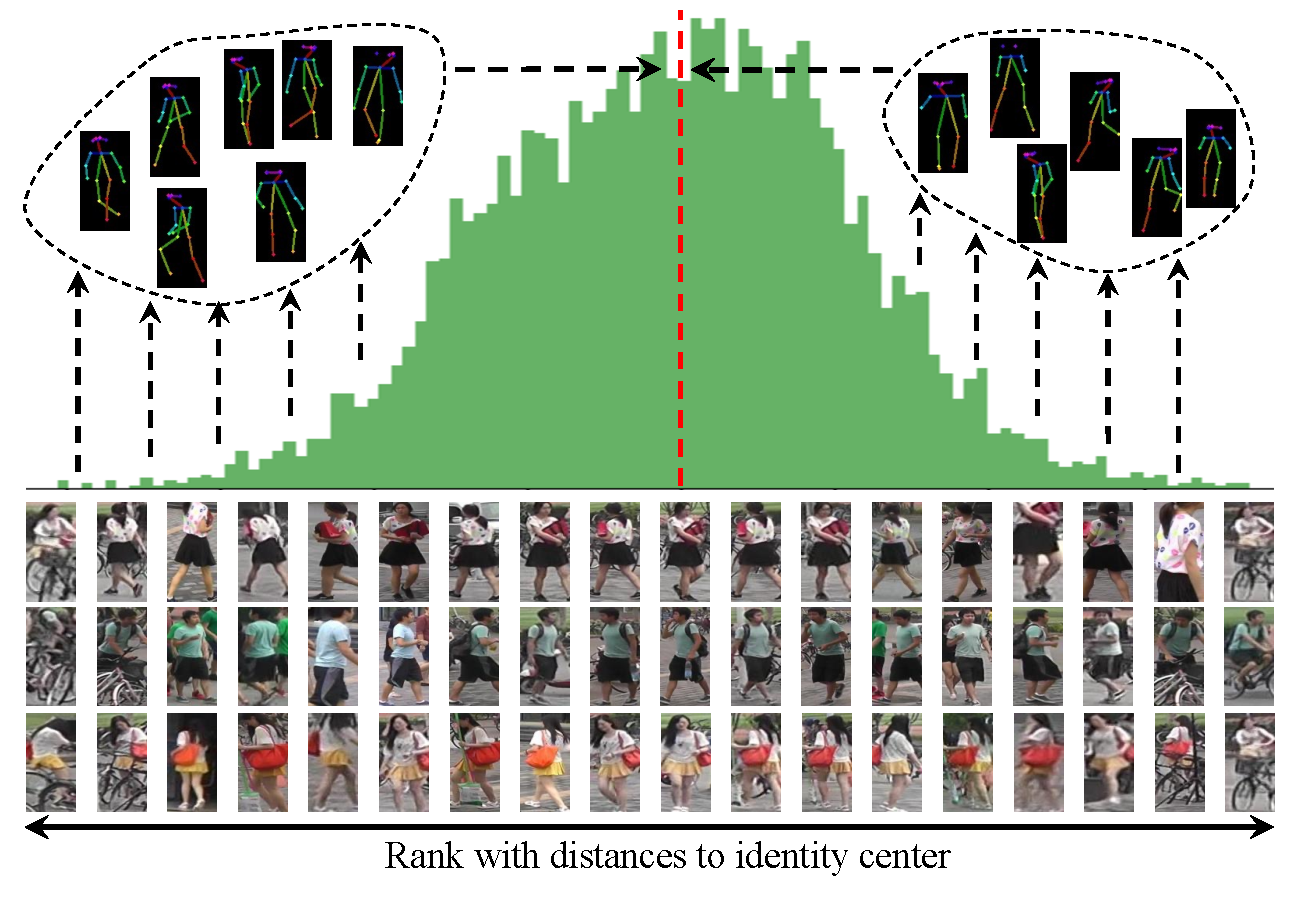
\includegraphics[width=0.85\linewidth]{figs/pdf/intro.pdf}
\caption{The real feature distribution of images from the same ID extracted by TransReID, and the main idea of our work is to make features closer/centralized to the ID center.}
\label{fig:intro}
\end{figure}

Thus, the main contributions of this paper include:
\begin{itemize}
    \item[$\bullet$]\textbf{Training-Free} \textbf{Feature Centralization} framework that can be directly applied to different ReID tasks/models, even an ImageNet pretrained ViT without ReID training;
    \item[$\bullet$]\textbf{I}dentity-Guided \textbf{P}edestrian \textbf{G}eneration (IPG) paradigm, leveraging identity features to generate high-quality images of the same identity in different poses to achieve feature centralization;
    \item[$\bullet$]\textbf{N}eighbor \textbf{F}eature \textbf{C}entralization (NFC) based on sample's neighborhood, discovering hidden positive samples from gallery/query set to achieve feature centralization.
\end{itemize}










% 行人重识别(Person Re-identification, ReID)任务是一个图像检索问题,目标是从行人图像中提取行人特征,并利用这些特征进行精确匹配与检索。当前的大部分研究集中在构建强大的特征提取模型上,通常通过增加模型参数和特征维度以便从有限数据中学习区分性特征。然而,在实际应用中,因图像质量或模型局限性,部分提取到的特征可能不属于行人身份本身,反而成为噪声特征。现有方法通常未关注噪声特征的存在,无法有效应对其影响。因此,如何有效抑制特征中的噪声并增强其身份表示能力,成为本文研究的关键问题。

% 特征噪声虽难以完全消除,但可以通过合适的方法予以削弱。基于此,我们提出了特征“身份中心化”的概念。得益于ReID模型的损失函数,训练过程自然会促使同一身份的样本特征逐渐收敛于特征空间中的一个聚集点,我们称之为“身份中心”。根据中心极限定理,当样本量足够大时,同一身份的特征会围绕这个隐式的身份中心呈正态分布。由此,可以通过叠加同一身份的特征,使得单个特征更接近其身份中心,从而弱化噪声并增强其身份代表性。

% 然而,如何获取相同身份的样本是一个挑战,因为我们通常无法直接获取每个样本的身份标签。最简单的就是水平反转来获得一个额外特征,这也是ReID领域中很多热你会用到的一个trick。此外,受到Re-rank机制的启发,我们可以通过特征的距离矩阵去挖掘潜在的正样本对特征进行中心化。但Re-rank是一种一次性的方法,通过加权,缩放等去修改特征或者距离矩阵,而我们进行特征增强后,会进行L2 norm来归一化,维持了特征的原有的分布。

% 当然,随着生成模型的快速发展,生成同一身份的不同姿态图像成为可能。例如,ABC等人尝试了基于GAN的生成方法,但生成效果有限,主要用于扩增训练数据。随着扩散模型在图像生成领域取得突破,CDF等人验证了生成同一人不同姿态高质量图像的可行性。然而,这些方法缺乏身份特征的指导,在行人图像生成中往往受到背景信息和遮挡物的干扰,难以保证不同姿态生成图像的身份一致性。

% 为了解决上述问题,本文提出了一种无需额外训练的行人ReID框架。本文的主要贡献包括:

% 详细分析了ReID特征的分布特性,提出了一种模型无关的特征增强框架,即使基于预训练的ViT模型也能直接应用于ReID任务;
% 提出了一个基于身份特征指导的行人图像生成框架,利用身份信息生成同一身份不同姿态的高质量图像,以实现特征增强;
% 设计了一种基于互惠信息挖掘的特征增强算法,从样本集中高效挖掘潜在信息以提升特征的身份表示能力。


% zheng等人的文章指出,即使图片质量再差,甚至不是一个“人”,其身份的预测最大概率仍然会落在其对应的identity上。在特征维度,任意两个样本,只要他们是来自同一个身份个体的,他们的特征空间总会有关联。

%-------------------------------------------------------------------------
